\documentclass{beamer}

\usepackage[english]{babel}
\usepackage{amsmath,amsthm,amsfonts}
\usepackage{xkeyval}
\usepackage{graphics}
\usepackage{url}
\usepackage[lined,boxed,linesnumbered]{algorithm2e}
\usepackage{CJKutf8}

\definecolor{mycolor}{RGB}{128,0,128}
\definecolor{mycolorlys}{RGB}{139,0,139}
\definecolor{mycolorlyslys}{RGB}{150,0,150}
\definecolor{mycolorlyslyslys}{RGB}{160,0,160}

\mode<presentation>
{
	\usetheme{Madrid}
	\usecolortheme[named=mycolor]{structure}
	\useinnertheme{rectangles}
	\useoutertheme{infolines}%default,infolines,miniframes,shadow,sidebar,smoothbars,smoothtree,split,tree
	\usefonttheme[onlymath]{serif}
	\setbeamercovered{transparent}
	\setbeamertemplate{blocks}[rounded][shadow=true]
}

\logo{
\includegraphics[scale=0.07]{images/HUSTLogo}}
\title{RBMs\&LR for Discrimination}
\author{Yunfei WANG}
\institute{\inst{1}School of Computer Science \& Technology \\ Huazhong University of Science \& Technology}
\date{May 20, 2013}

\begin{document}
\begin{CJK*}{UTF8}{gbsn}

\begin{frame}
\titlepage
\end{frame}

\begin{frame}\frametitle{Table of contents}
\tableofcontents
\end{frame}

\section{Using RBMs for Discrimination}
\subsection{Strategy One}
\begin{frame}\frametitle{Using Hidden Features directly}
\begin{block}{\textcolor{magenta}{Hidden Features}+\textcolor{red}{Discriminative Methods}}
\centering
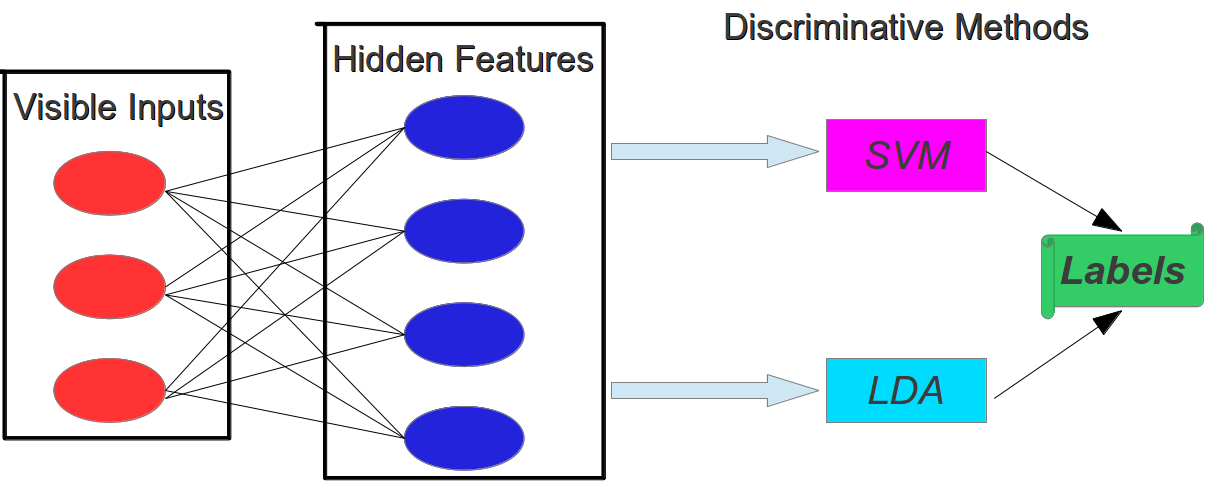
\includegraphics[scale=0.27]{images/pic1}
\end{block}
\end{frame}

\subsection{Strategy Two}
\begin{frame}\frametitle{Train RBM for each class}
Log probability for visible vector of RBM trained on class $c$:
\begin{equation}
\log p(v|c)=-F_c(v)-\log Z_c
\end{equation}
where $F_c(v)$ is free energy of visible vector,$Z_c$ is partition function of RBM for class $c$ which is different for each class-specific RBM.
\begin{center}
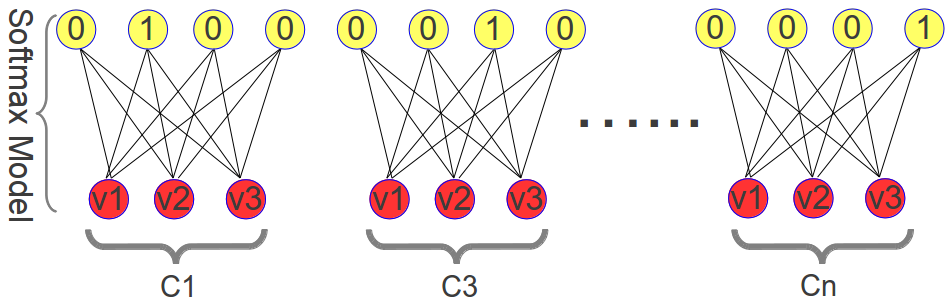
\includegraphics[scale=0.2]{images/pic2}
\end{center}
Predict class from free energy of all class-specific RBMs:
\begin{equation}
\log p(c|v)=\frac{\exp(-F_c(v)-\log\hat{Z}_c)}{\sum_d\exp(-F_d(v)-\log\hat{Z}_d)}
\end{equation}
\end{frame}

\subsection{Strategy Three}
\begin{frame}\frametitle{Train a joint density model}
A joint density model using a single RBM with two sets of visible units:
\begin{center}
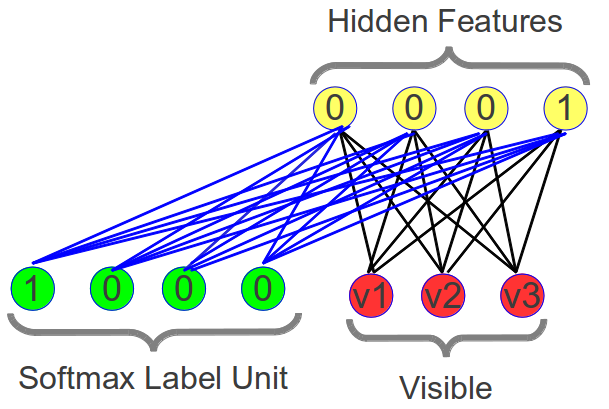
\includegraphics[scale=0.23]{images/pic3}
\end{center}
The probability of picking the $c$th class:
\begin{equation}
\log p(c|v)=\frac{\exp(-F_c(v))}{\sum_d\exp(-F_d(v))}
\end{equation}
Partition function is same for all classes.Apparently,the one with lowest free energy is chosen as the most likely class.
\end{frame}

\subsection{Computing Free Energy}
\begin{frame}\frametitle{Free Energy for visible vector}
The energy of each pair of visible vector $v$ and hidden vector $h$:
\begin{equation}
E(v,h)=-v^TWh-a^Tv-b^Th
\end{equation}
We have the following equation:
\begin{equation}
\begin{split}
\exp(-F(v))=&\sum_h\exp(-E(v,h))\\
&=\exp(a^Tv)\sum_h\exp(v^TWh+b^Th)\\
&=\exp(a^Tv)\prod_j\sum_{h_j\in\{0,1\}}\exp(\sum_iW_{ij}h_j+b_jh_j)\\
&=\exp(a^Tv)\prod_j(1+\exp(\sum_iv_iW_{ij}+b_j))
\end{split}
\end{equation}
\textcolor{blue}{\emph{Free Energy}} of $v$:$F(v)=-\sum_iv_ia_i-\sum_j\log(1+\exp(\sum_iv_iW_{ij}+b_j))$.
\end{frame}

\section{Logistic Regression(LR) for Discriminant}
\subsection{Binary Case}
\begin{frame}\frametitle{Binary Case}
Given two classes $C_1$ and $C_2$,transform linear decision function $y(x)=w^Tx+b$ to model class-belonging probabilities $P(C_i|x)$:
\begin{equation}
y(x)=\log(\frac{P(C_1|x)}{P(C_2|x)})\Longrightarrow P(C_1|x)=\frac{1}{1+e^{-y(x)}}=\frac{1}{1+e^{-(w^Tx+b)}}
\end{equation}
Assume training data $x_1,\cdots,x_n$ form a random sample from a sequence of $n$ Bernoulli trails,the likelihood of observation $y_1,\cdots,y_n$ is:
\begin{equation}
L=\prod_{j=1}^nP(C_1|x_j)^{y_j}(1-P(C_1|x_j))^{1-y_j}
\end{equation}
Add extra regularisation term to avoid overfitting and instability:
\begin{equation}
\log L=\sum_{j=1}^n\left[{y_j}P(C_1|x_j)+(1-y_j)(1-P(C_1|x_j))\right]-\lambda\|w\|
\end{equation}
\end{frame}
\subsection{Multiclass Situation}
\begin{frame}\frametitle{Multiclass Situation}
For multinominal LR with $k$ classes,the decision function takes the following form:
\begin{equation}
P(C_i|x)=\frac{exp(w_i^Tx)}{\sum_j\exp(w_j^Tx)}
\end{equation}
where $\exp(w_i^Tx)$ is proportional to $P(C_i|X)$ under binary case.\\
\textcolor{blue}{Optimize weight vectors $w_j$}:One-against-All or Pairwise.\\
\textcolor{red}{Insight into posterior probability and geometric location:}
\begin{center}
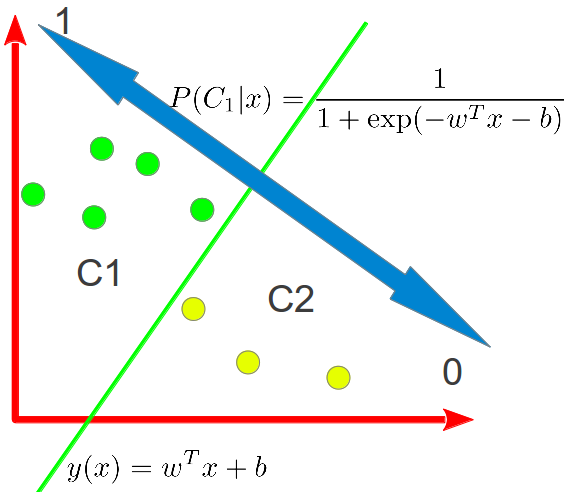
\includegraphics[scale=0.25]{images/pic4}
\end{center}
\end{frame}

\section{Experiments}
\begin{frame}
\begin{figure}
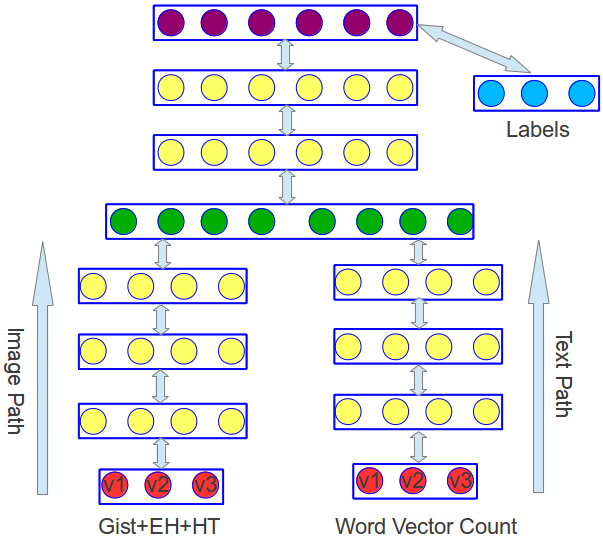
\includegraphics[scale=0.3]{images/pic5}
\caption{Framework of Processing}
\end{figure}
\end{frame}
\end{CJK*}
\end{document}